\documentclass{article}

\usepackage[spanish]{babel}
\usepackage{titling}
\usepackage{graphicx}
\usepackage{graphicx}
\usepackage[export]{adjustbox}
\usepackage{hyperref}
\usepackage{ragged2e}
\usepackage{indentfirst}
\usepackage{float}
\usepackage{microtype}

\title{Universidad Nacional de Córdoba\\Facultad de Ciencias Exactas, Físicas y Naturales}
\author{Tomas Sarquis}
\date{Agosto 2020}

\newcommand{\fnuml}{\emph{Unified Modeling Language}, \url{en.wikipedia.org/wiki/Unified_Modeling_Language}}
\newcommand{\fnpipe}{\url{http://pipe2.sourceforge.net}}
\newcommand{\fndoc}{La documentación se encuentra en el archivo \emph{html} "documentacion/html/index.html"}
\newcommand{\fndoxy}{\url{www.doxygen.nl}}
\newcommand{\fninv}{src/T-Invariantes.txt}
\newcommand{\fninverr}{src/T-InvariantesErr.txt}
\newcommand{\fnpruebas}{informe/pruebas.ods}

\hypersetup{
    colorlinks,
    citecolor=black,
    filecolor=black,
    linkcolor=black,
    urlcolor=black
}

\begin{document}
    %%%%%%%%%%%%%%%%%%%%%%%%%%%%%%%%%%%%%%%%%%%%%%%%%%%%%%%%%%%%%%%%%%%%%%%%%%%%%%%%%%%%%%%%
    \begin{titlingpage}
        \maketitle
        \null \null \null \null
        \begin{center}
            {\huge Programación Concurrente}
        \end{center}
        \topskip0pt
        \vspace*{\fill}
        \justify
        El presente documento detalla la realización del \textbf{trabajo práctico número 3} 
        de la asignatura \textbf{programación concurrente}, correspondiente al año \textbf{2019}
        por el alumno Tomas Sarquis, matrícula 39884977
        \vspace*{\fill}
    \end{titlingpage}
    \tableofcontents 
    %%%%%%%%%%%%%%%%%%%%%%%%%%%%%%%%%%%%%%%%%%%%%%%%%%%%%%%%%%%%%%%%%%%%%%%%%%%%%%%%%%%%%%%%
    \newpage
    \section{Introducción}
    %%%%%%%%%%%%%%%%%%%%%%%%%%%%%%%%%%%%%%%%%%%%%%%%%%%%%%%%%%%%%%%%%%%%%%%%%%%%%%%%%%%%%%%%
    \subsection{Objetivo}
    El objetivo del siguiente trabajo práctico es que el estudiante sea capaz de diseñar,
    implementar y analizar un programa que realice una simulación mediante redes de Petri,
    conociendo sus propiedades y monitorizando que éstas se cumplan. \par
    Algunos de los conocimientos aplicados en este trabajo son:
    \begin{itemize}
        \item Programación en \emph{Java}
        \item Concurrencia y manejo de hilos en \emph{Java}
        \item Redes de Petri: propiedades y ventajas
        \item \emph{UML}\footnote{\fnuml}: diagramas para modelar
    \end{itemize}
    %%%%%%%%%%%%%%%%%%%%%%%%%%%%%%%%%%%%%%%%%%%%%%%%%%%%%%%%%%%%%%%%%%%%%%%%%%%%%%%%%%%%%%%%
    \subsection{Enunciado}
    Se debe implementar un simulador de un procesador con dos núcleos. A partir de la red de
    Petri de la \emph{figura 1}, la cual representa a un procesador mono-núcleo, se deberá 
    extender la misma a una red que modele un procesador con dos núcleos. Además, se debe
    implementar una política que resuelva los conflictos que se generan con las transiciones
    que alimentan los buffers de los núcleos.
    \begin{figure}[H]
        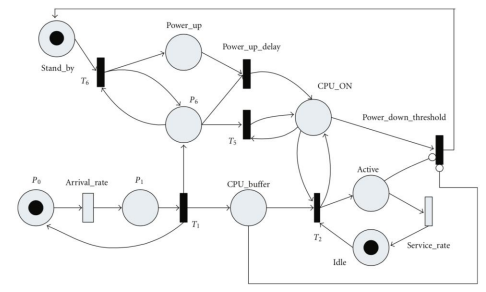
\includegraphics[width=0.9\textwidth, center]{rdp_enun.png}
        \caption{Red de Petri mono-núcleo}
    \end{figure} 
    %%%%%%%%%%%%%%%%%%%%%%%%%%%%%%%%%%%%%%%%%%%%%%%%%%%%%%%%%%%%%%%%%%%%%%%%%%%%%%%%%%%%%%%%
    \newpage
    \section{Implementación}
    %%%%%%%%%%%%%%%%%%%%%%%%%%%%%%%%%%%%%%%%%%%%%%%%%%%%%%%%%%%%%%%%%%%%%%%%%%%%%%%%%%%%%%%%
    \subsection{Red de Petri}
    En la \emph{figura 2} se observa cómo fue modelada la red de Petri de acuerdo al enunciado. \par
    La red de Petri modelada cuenta con:
    \begin{itemize}
        \item 16 plazas
        \item 15 transiciones
    \end{itemize}
    \begin{figure}[H]
        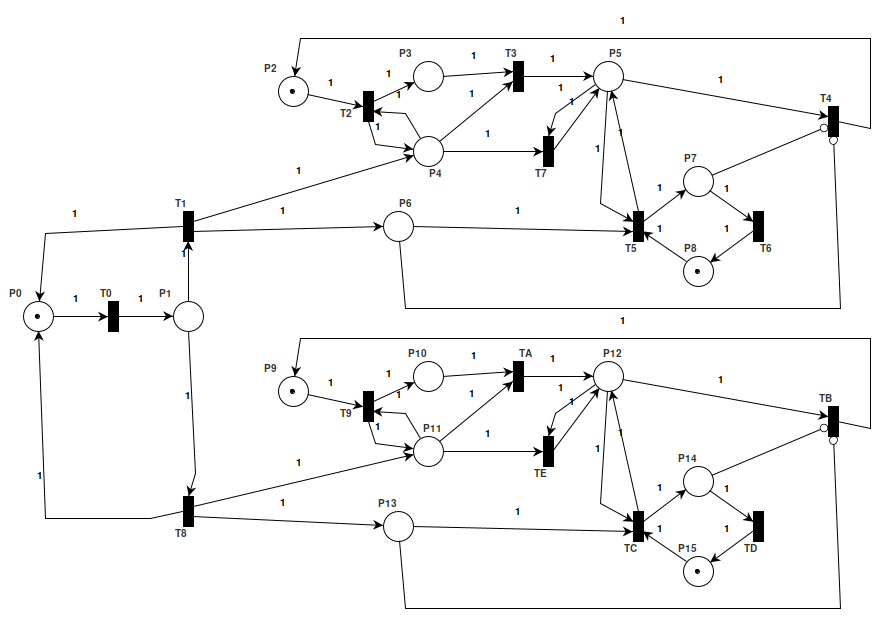
\includegraphics[width=0.9\textwidth, center]{rdp.png}
        \caption{Red de Petri doble núcleo}
    \end{figure}   
    %%%%%%%%%%%%%%%%%%%%%%%%%%%%%%%%%%%%%%%%%%%%%%%%%%%%%%%%%%%%%%%%%%%%%%%%%%%%%%%%%%%%%%%%
    \subsection{Hilos}
    Teniendo en cuenta la red de la \emph{figura 2}, lo siguiente es pensar cuántos hilos
    serán los encargados de ejecutarse en el programa. \par
    Luego de realizar un análisis, se llegó a la conclusión de que en la red deben trabajar
    \textbf{7 hilos} en forma concurrente. Estos hilos son llamados:
    \begin{itemize}
        \item ProcessGenerator
        \item CPUPower x 2
        \item CPUProcessing x 2
        \item CPUGarbageCollector x 2
    \end{itemize}
    \textbf{ProcessGenerator:} Encargado de generar los procesos comunes a ambos CPUs.
    Dispara las transiciones 0, 1 y 7. \newline \newline
    \textbf{CPUPower:} Maneja el encendido/apagado de cada CPU. Dispara las transiciones
    2, 3 y 4 o 8, 9 y A. \newline \newline
    \textbf{CPUProcessing:} Procesa las tareas de cada CPU. Dispara las transiciones
    5 y 6 o B y C. \newline \newline
    \textbf{CPUGarbageCollector:} Previene que no se junten \emph{tokens} "basura". 
    Dispara las transiciones E o D.\newline \par
    Cabe destacar que las letras \{\textbf{A, B, C, D, E}\}, en éstas últimas entradas, 
    equivalen a las transiciones \{\textbf{10, 11, 12, 13, 14}\}. 
    %%%%%%%%%%%%%%%%%%%%%%%%%%%%%%%%%%%%%%%%%%%%%%%%%%%%%%%%%%%%%%%%%%%%%%%%%%%%%%%%%%%%%%%%
    \subsection{Clases en Java}
    El programa encargado de simular el sistema se desarrolla en el lenguaje de programación
    \emph{Java}. \par
    A continuación, se describen las clases, implementadas en dicho lenguaje,
    que modelan el sistema:
    \begin{itemize}
        \item \textbf{Cola:} Colas (\emph{queues}), las cuales son usadas para que los
        hilos puedan dormir en caso que lo necesiten
        \item \textbf{Colors:} Clase sin funciones que contiene códigos de colores (para 
        loggear)
        \item \textbf{CPUGarbageCollector:} Modelo del hilo CPUGarbageCollector anteriormente
        descrito
        \item \textbf{CPU:} Modela un CPU. Clase encargada de comunicar los hilos Generator,
        Processing y GarbageCollector
        \item \textbf{CPUPower:} Modelo del hilo CPUPower anteriormente descrito
        \item \textbf{CPUProcessing:} Modelo del hilo CPUProcessing anteriormente descrito
        \item \textbf{Main:} Clase principal y ejecutable
        \item \textbf{Monitor:} Encargada de administrar los tiempos y el uso de la red de 
        Petri
        \item \textbf{Politica:} A la hora de despertar un hilo, la política es quien decide
        a cuál hacerlo
        \item \textbf{ProcessBuffer:} Modelo de un buffer en el cuál se depositan Process
        \item \textbf{ProcessGenerator:} Modelo del hilo ProcessGenerator anteriormente
        descrito
        \item \textbf{Process:} Clase que simula un proceso de CPU. Dichos Process van a
        parar a un ProcessBuffer
        \item \textbf{RedDePetri:} Implementación de la red de Petri
        \item \textbf{XMLParser:} Parsea las características de la red de Petri desde un
        archivo \emph{xml}
    \end{itemize} \par
    \begin{figure}[H]
        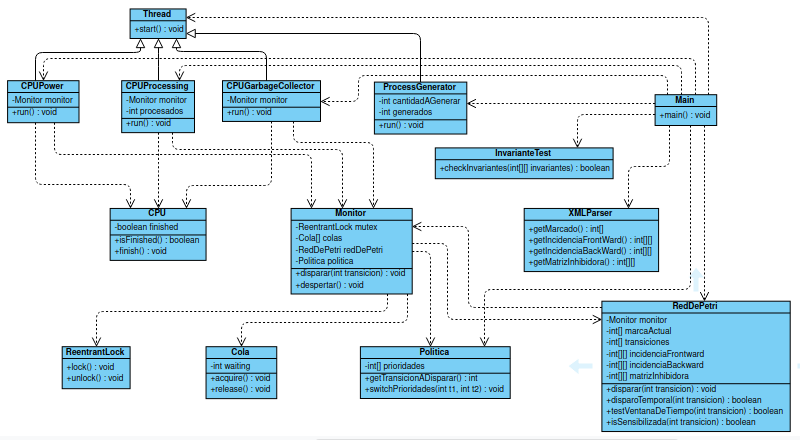
\includegraphics[width=0.9\textwidth, center]{diagrama-clases.png}
        \caption{Diagrama de clases simplificado}
    \end{figure}
    Varios métodos y/o atributos fueron omitidos para mayor claridad en el diagrama de clases
    de la \emph{figura 3}. \par   
    Para información más detallada acerca de las clases y  sus funciones, se puede consultar
    la documentación\footnote{\fndoc} hecha por \emph{Doxygen}\footnote{\fndoxy}.
    %%%%%%%%%%%%%%%%%%%%%%%%%%%%%%%%%%%%%%%%%%%%%%%%%%%%%%%%%%%%%%%%%%%%%%%%%%%%%%%%%%%%%%%%
    \subsection{Monitor}
    La clase \emph{Monitor} es la que se encarga de administrar los hilos de nuestro programa.
    A continuación, para un mejor entendimiento de la clase, se observa un diagrama de secuencia
    que ilustra cómo un hilo entra al monitor, hace su trabajo y sale del mismo.
    \begin{figure}[H]
        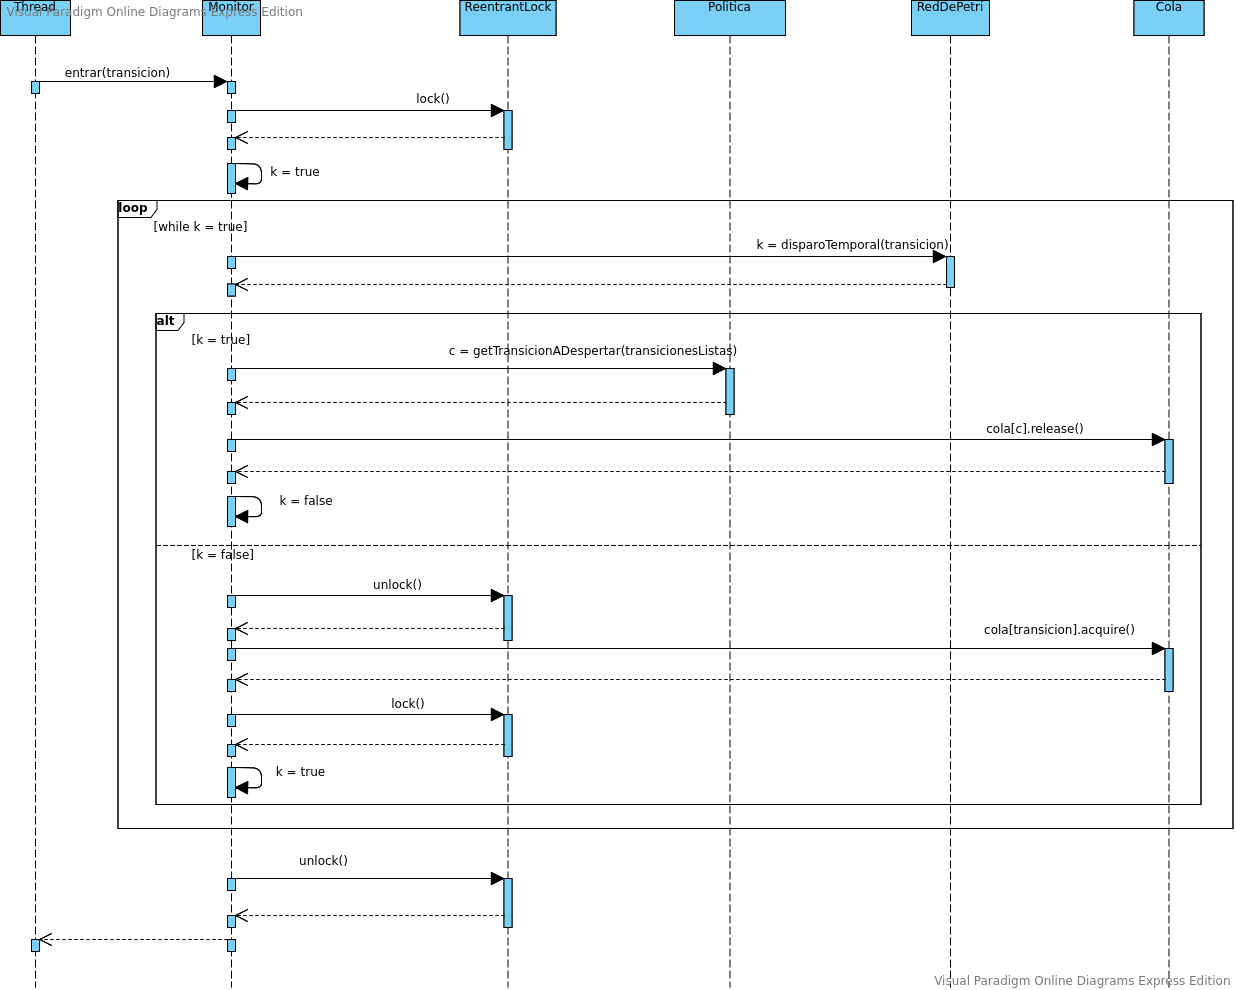
\includegraphics[width=1.2\textwidth, center]{secuencia-monitor.png}
        \caption{Diagrama de secuencia del monitor}
    \end{figure}
    %%%%%%%%%%%%%%%%%%%%%%%%%%%%%%%%%%%%%%%%%%%%%%%%%%%%%%%%%%%%%%%%%%%%%%%%%%%%%%%%%%%%%%%%
    \subsection{Política}
    La clase \emph{política} se encarga de facilitar la elección de a qué hilo despertar en 
    el caso en que haya más de uno durmiendo. \par
    La forma de hacer esto es mediante prioridades: se le asigna una prioridad \textbf{distinta}
    a cada una de las transiciones de la red. \par
    Cuando queramos hacer uso de la política, simplemente le indicamos cuáles son las
    transiciones listas para dispararse y ella nos indicará cuál de esas transiciones es la
    que tiene la mayor prioridad. \par
    Además, la clase \emph{política} cuenta con un método capaz de intercambiar prioridades
    entre dos transiciones. Esto podría ser útil, en el caso en que se quiera depositar más
    tareas en un CPU que en el otro.
    %%%%%%%%%%%%%%%%%%%%%%%%%%%%%%%%%%%%%%%%%%%%%%%%%%%%%%%%%%%%%%%%%%%%%%%%%%%%%%%%%%%%%%%%
    \subsection{Invariantes}
    Sabemos que una de las maneras de chequear que la red (y nuestro programa) funciona 
    de forma correcta, es analizando las invariantes. Estas son, las \textbf{t-invariantes}
    y las \textbf{p-invariantes}. \par
    Para el análisis, se usó la herramienta Pipe\footnote{\fnpipe}.
    Los resultados fueron los siguientes: \newline \newline
    \textbf{P-Invariantes:} \\
    \begin{figure}[H]
        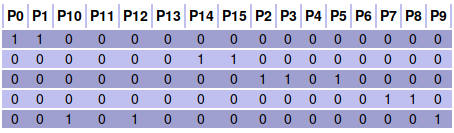
\includegraphics[width=0.7\textwidth, center]{p-invariante.png}
        \caption{Análisis de P-Invariantes en Pipe}
    \end{figure}
    La \emph{figura 5} nos enseña qué plazas están relacionadas mediante una invariante de
    plazas. Esta relación indica que la suma de los \emph{tokens} en dichas plazas, en cada
    relación, sea siempre unitaria. Estos es: \newline \newline
    \begin{center}
        $M(P0) + M(P1) = 1$ \newline \newline
        $M(P14) + M(P15) = 1$ \newline \newline
        $M(P2) + M(P3) + M(P5) = 1$ \newline \newline
        $M(P10) + M(P12) + M(P9) = 1$ \newline \newline
    \end{center} \par
    Para comprobar que lo anterior se cumpla siempre, la clase \emph{RedDePetri} hace un 
    chequeo cada vez que se dispara una transición. El método de la clase que hace dicho
    chequeo se llama \emph{isPInvariantesCorrecto}. \newline \newline
    \textbf{T-Invariantes:} \newline \par
    De la misma forma, podemos observar en la \emph{figura 6} las invariantes de transición
    que existen en nuestro sistema. \\
    \begin{figure}[H]
        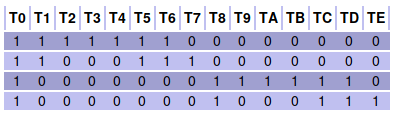
\includegraphics[width=0.7\textwidth, center]{t-invariante.png}
        \caption{Análisis de T-Invariantes en Pipe}
    \end{figure}
    Para este análisis, la clase \emph{Main} se encarga de grabar todas las transiciones 
    (en orden) que han sido disparadas en un archivo\footnote{\fninv} de texto. Luego, un
    programa en Python (\emph{InvariantesTest.py}) usa esa información para, mediante un 
    algoritmo de remplazo con regex, ir eliminando las coincidencias (o \emph{matches}) 
    entre el \emph{log} de transiciones y las invariantes. Si el sistema funciona 
    correctamente, deben quedar eliminadas todas las transiciones. \newline \par
    Se realizó un análisis en los \emph{softwares} Charlie/Snoopy para respaldarnos nó 
    solamente en Pipe. En este análisis consideramos un CPU mono-core. Los resultados 
    fueron los mismos:
    \begin{figure}[H]
        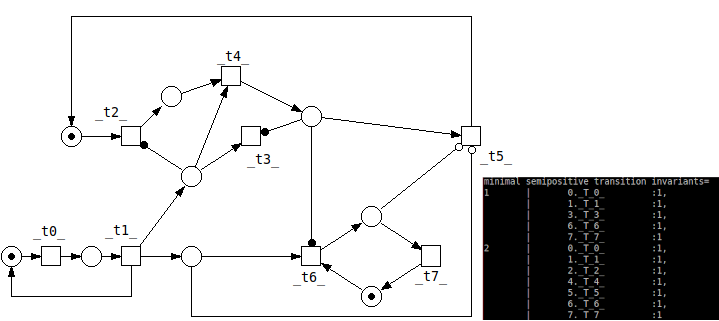
\includegraphics[width=1.0\textwidth, center]{t-invariante-snoopy.png}
        \caption{Análisis de T-Invariantes en Charlie/Snoopy}
    \end{figure}
    %%%%%%%%%%%%%%%%%%%%%%%%%%%%%%%%%%%%%%%%%%%%%%%%%%%%%%%%%%%%%%%%%%%%%%%%%%%%%%%%%%%%%%%%
    \newpage
    \section{Resultados}
    %%%%%%%%%%%%%%%%%%%%%%%%%%%%%%%%%%%%%%%%%%%%%%%%%%%%%%%%%%%%%%%%%%%%%%%%%%%%%%%%%%%%%%%%
    \subsection{Análisis de invariantes}
    \textbf{P-invariantes: } el análisis de las invariantes de plaza consiste en chequear, 
    cada vez que se dispara una transición, que las ecuaciones de la sección 2.5 se cumplen.
    No hubo mayor problema con las mismas, comprobándose que el análisis siempre indica que
    las invariantes de plaza se llevan a cabo correctamente. \par
    Los resultados de dicho análisis se muestran al finalizar cada ejecución del programa.
    \newline \par
    \textbf{T-invariantes: } el análisis de las invariantes de transicion consiste en 
    observar el log de transiciones e ir remplazando las invariantes que van coincidiendo.
    Como se dijo anteriormente, éste análisis se realizó en Python haciendo uso de la 
    librería de regex. \par
    Se tuvieron en cuenta dos métodos distintos de análisis. Debido a esto, el programa 
    consta de dos funciones de interés: \par
    \begin{itemize}
        \item test\_colectivo\_4inv(): Se realiza el análisis con las invariantes obtenidas 
        por Pipe. Se hace un reemplazo recursivo hasta que no haya más coincidencias.
        \begin{figure}[H]
            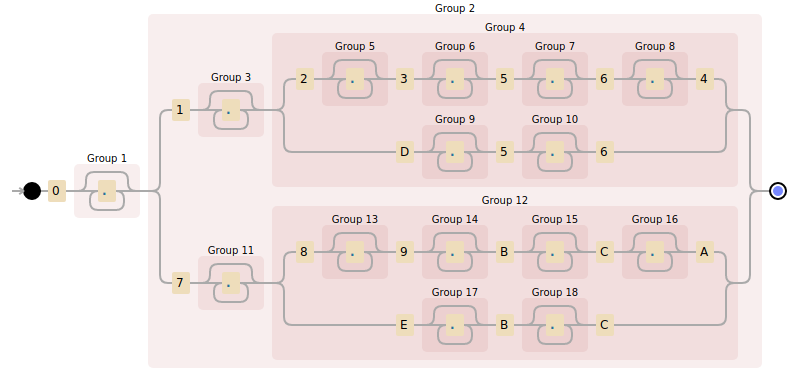
\includegraphics[width=0.9\textwidth, center]{regex4inv.png}
            \caption{Regex utilizado en la función de 4 invariantes}
        \end{figure}
        \item test\_colectivo\_2inv(): Se realiza el análisis con dos invariantes escogidas 
        por el diseñador. Se hace un reemplazo recursivo hasta que no haya más coincidencias.
        Luego, se reemplazan las transiciones equivalentes al \emph{GarbageCollector}.
        \begin{figure}[H]
            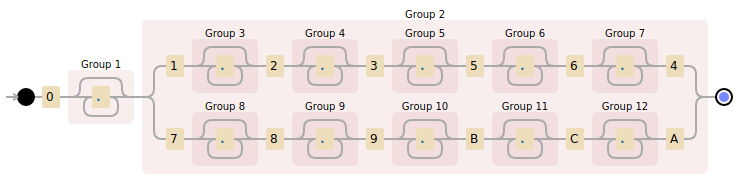
\includegraphics[width=0.9\textwidth, center]{regex2inv.png}
            \caption{Regex utilizado en la función de 2 invariantes}
        \end{figure}
    \end{itemize} \par
    Recordar que las letras \{\textbf{A, B, C, D, E}\}, en éstas últimas imágenes, 
    equivalen a las transiciones \{\textbf{10, 11, 12, 13, 14}\}. \newline \newline
    \textbf{Resultados}
    \begin{center}
        \begin{table}[H]
            \centering
            \begin{tabular}{||c|c|c|c||} 
                \hline
                Procesos & Trans. totales & Trans. restantes (4inv) & Trans. restantes (2inv) \\ [0.5ex] 
                \hline\hline
                250 & 1486 & 17 & 373 \\ 
                \hline
                500 & 2984 & 24 & 771 \\
                \hline
                750 & 4478 & 22 & 1183 \\
                \hline
                1000 & 5956 & 24 & 1527 \\
                \hline
                1250 & 7430 & 17 & 2008 \\
                \hline
                1500 & 8938 & 19 & 2434 \\
                \hline
            \end{tabular}
            \caption{Resultados de análisis de T-Invariantes}
        \end{table}
    \end{center} \par
    Cabe destacar que para éste análisis se tuvo SERVICERATE = ARRIVALRATE = 10 [ms]. \par
    Como se puede ver, en ambos casos \textbf{hay transiciones restantes}. Obviamente no es
    lo deseado. \par
    En el caso del método de \textbf{2 invariantes}, las transiciones restantes son muchas.
    Esto era esperado, ya que el método no contempla que, cada vez que se procesa una tarea,
    no necesariamente el CPU se enciende/apaga. \par
    En el caso del método de \textbf{4 invariantes}, se esperaba que las transiciones 
    restantes sean nulas. Si bien esto no es asi, podemos observar que la cantidad de 
    transiciones restantes no aumenta con la cantidad de transiciones totales, si no, que se
    mantienen en el mismo rango de valores. \newline \par 
    A pesar de que los análisis indican que el programa funciona de forma incorrecta, se
    invita al lector a leer la sección del apéndice \textbf{Caso de análisis}. En dicha 
    sección, se demuestra el correcto funcionamiento del programa.
    %%%%%%%%%%%%%%%%%%%%%%%%%%%%%%%%%%%%%%%%%%%%%%%%%%%%%%%%%%%%%%%%%%%%%%%%%%%%%%%%%%%%%%%%
    \subsection{Tiempos}
    A continuación, en el \emph{cuadro 2}, se describen los tiempos que lleva el programa en 
    ejecutarse. Los tiempos de la red son los siguientes: \par
    \begin{itemize}
        \item \emph{ArrivalRate} = 10 [ms]
        \item \emph{ServiceRate} = 15 [ms]
        \item \emph{StandByDelay} = 30 [ms]
    \end{itemize} 
    \begin{center}
        \begin{table}[H]
            \centering
            \begin{tabular}{||c|c||} 
                \hline
                Procesos & Tiempo de ejecución (\emph{avg}) \\ [0.5ex] 
                \hline\hline
                500 & 2,59 \\ 
                \hline
                1000 & 5,16 \\
                \hline
                1500 & 7,76 \\
                \hline
                2000 & 10,35 \\
                \hline
                2500 & 12,95 \\
                \hline
                3000 & 15,53 \\
                \hline
                3500 & 18,13 \\
                \hline
                4000 & 20,74 \\
                \hline
            \end{tabular}
            \caption{Resultados de análisis. Cada fila equivale a 5 muestras}
        \end{table}
    \end{center}
    \begin{figure}[H]
        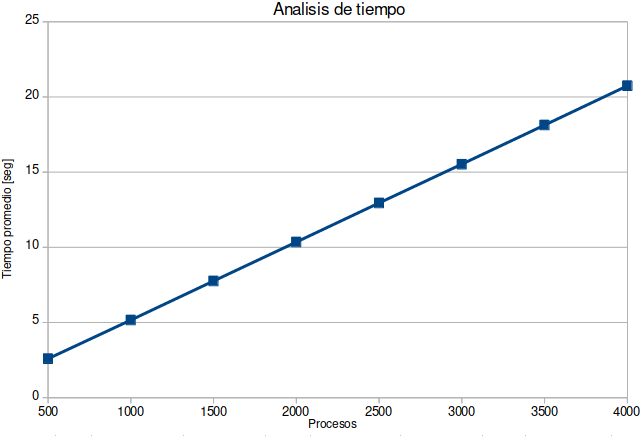
\includegraphics[width=0.9\textwidth, center]{tiempos.png}
        \caption{Gráfica de cantidad de procesos vs tiempos}
    \end{figure}
    Se observa una clara linealidad a medida que aumenta la cantidad de procesos.
    %%%%%%%%%%%%%%%%%%%%%%%%%%%%%%%%%%%%%%%%%%%%%%%%%%%%%%%%%%%%%%%%%%%%%%%%%%%%%%%%%%%%%%%%
    \newpage 
    \section{Conclusión}
    %%%%%%%%%%%%%%%%%%%%%%%%%%%%%%%%%%%%%%%%%%%%%%%%%%%%%%%%%%%%%%%%%%%%%%%%%%%%%%%%%%%%%%%%
    En el presente trabajo práctico se llevó a cabo la implementación de un sistema que modela
    dos procesadores trabajando concurrentemente, orquestados por una red de Petri. Esta última
    nos da la ventaja de poder controlar que el sistema funcione correctamente, chequeando que
    las propiedades de la red sean las correctas. Además, el uso de redes de Petri nos da la 
    posibilidad de escalar nuestro sistema sin mayores problemas. \par
    Si bien me he encontrado con problemas (sección Resultados - Invariantes), se pudo 
    comprobar, por otros medios, que el sistema de verdad funciona de forma correcta. \par
    Dichos problemas se han intentado de resolver desde distintos frentes, no pudiéndose 
    lograr.
    %%%%%%%%%%%%%%%%%%%%%%%%%%%%%%%%%%%%%%%%%%%%%%%%%%%%%%%%%%%%%%%%%%%%%%%%%%%%%%%%%%%%%%%%
    \newpage 
    \section{Apéndice}
    %%%%%%%%%%%%%%%%%%%%%%%%%%%%%%%%%%%%%%%%%%%%%%%%%%%%%%%%%%%%%%%%%%%%%%%%%%%%%%%%%%%%%%%%
    \subsection{Repositorio del proyecto} \noindent
    Dirección: \url{https://github.com/sarquis88/final-concurrente}
    %%%%%%%%%%%%%%%%%%%%%%%%%%%%%%%%%%%%%%%%%%%%%%%%%%%%%%%%%%%%%%%%%%%%%%%%%%%%%%%%%%%%%%%%
    \subsection{Variables globales del programa} \noindent
    Las siguientes variables se encuentran en la clase \emph{Main} del programa:
    \begin{itemize}
        \item \textbf{CANTIDADPROCESOS}: cantidad de procesos a generar 
        \item \textbf{ARRIVALRATE}: tiempo \emph{alpha} de la llegada de nuevos procesos
        \item \textbf{SERVICERATE}: tiempo \emph{alpha} de procesamiento general
        \item \textbf{FACTORA}: factor de multiplicación del tiempo de procesamiento para el
        CPU A
        \item \textbf{FACTORB}: factor de multiplicación del tiempo de procesamiento para el
        CPU B
        \item \textbf{STANDBYDELAY}: tiempo \emph{alpha} del encendido de los CPUs
        \item \textbf{DUALCORE}: activación de \emph{dual core}
        \item \textbf{LOGGING}: activación de mensajes en consola
        \item \textbf{REALBUFFER}: activación de bufferes \emph{ProcessBuffer}
    \end{itemize}
    %%%%%%%%%%%%%%%%%%%%%%%%%%%%%%%%%%%%%%%%%%%%%%%%%%%%%%%%%%%%%%%%%%%%%%%%%%%%%%%%%%%%%%%%
    \subsection{Caso de análisis} \noindent
    A continuación, se demuestra el correcto funcionamiento del sistema, para un caso particular
    en el cuál se procesan 8 tareas:
    \begin{center}
        \begin{table}[H]
            \centering
            \begin{tabular}{||c|c|c|c||} 
                \hline
                Procesos & Trans. totales & Trans. restantes (4inv) & Trans. restantes (2inv) \\ [0.5ex] 
                \hline\hline
                8 & 48 & 5 & 10 \\ 
                \hline
            \end{tabular}
            \caption{Resultados de análisis de T-Invariantes. Caso de análisis}
        \end{table}
    \end{center} \par
    En el cuadro anterior, se observan los resultados negativos del análisis de 
    T-Invariantes. Las transiciones disparadas en éste caso, son: \newline 
    \begin{center}
        078901B2C35A6401072801079BCBE07E07E356D5CBCB64CA 
    \end{center} \par
    Se invita al lector, interesado, en chequear que dichas transiciones sean válidas para 
    nuestra red de Petri. Para ésto, se debe simular la anterior secuencia de transiciones
    en algún \emph{software} como Pipe.
    %%%%%%%%%%%%%%%%%%%%%%%%%%%%%%%%%%%%%%%%%%%%%%%%%%%%%%%%%%%%%%%%%%%%%%%%%%%%%%%%%%%%%%%%
\end{document}
